\documentclass{article}
% \usepackage[utf8]{inputenc}
\usepackage{tikz}
\usepackage{lipsum}
\usetikzlibrary{positioning}
\usepackage{pgfplots}
\usetikzlibrary{shapes.geometric, arrows, automata}

\begin{document}
\begin{tikzpicture}
 \node[draw,shape=rectangle] at (1,1) {A};
     \draw (0,0) -- (5,0) -- (5,5) -- (0,5) -- cycle;
\end{tikzpicture} 

\begin{tikzpicture}
 \node[draw,shape=rectangle] at (1,1) {B};
     \draw[gray] (0,0) grid (4,4);
     \draw[->] (0,0) -- (5,0) node[below] {$x$};
     \draw[->] (0,0) -- (0,5) node[left] {$y$};
\end{tikzpicture}

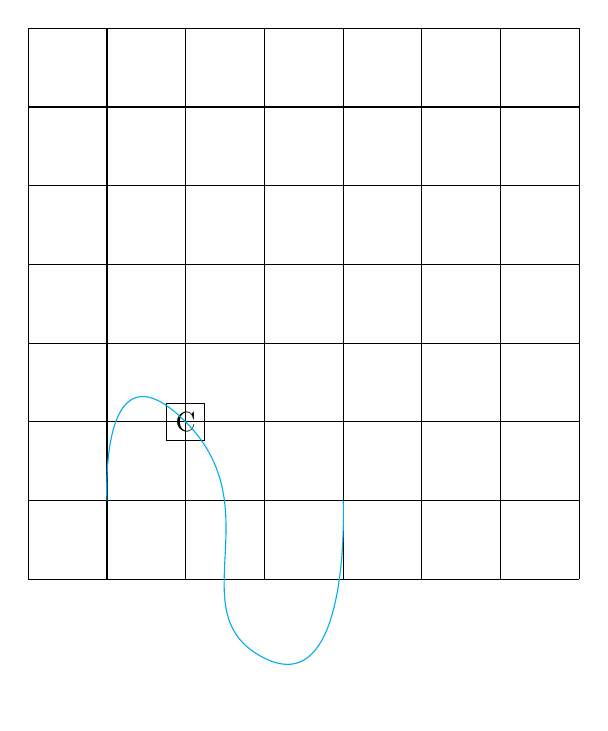
\begin{tikzpicture}
 \node[draw,shape=rectangle] at (1,1) {C};
     \draw (-1,-1) grid (6,6);
\draw [cyan, xshift=0cm] plot [smooth, tension=2] coordinates { (0,0) (1,1) (2,-2) (3,0)};
\end{tikzpicture}

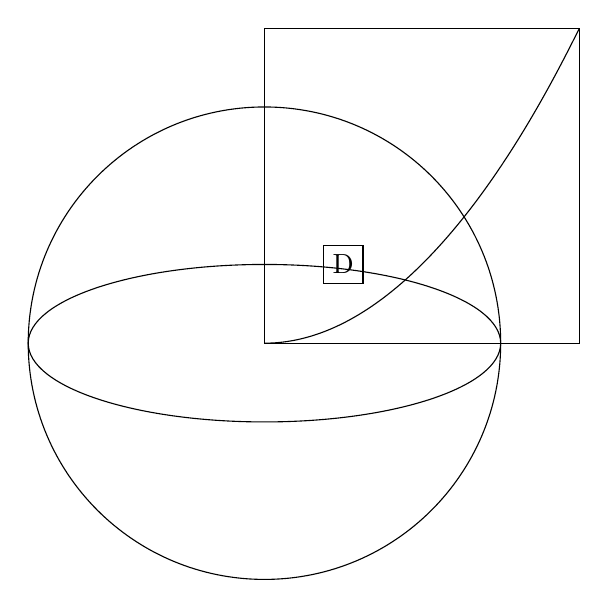
\begin{tikzpicture}
 \node[draw,shape=rectangle] at (1,1) {D};
     \draw (0,0) rectangle (4,4);
     \draw (0,0) parabola (4,4);
     \draw (0,0) circle (3cm);
     \draw (0,0) ellipse (3cm and 1cm);
\end{tikzpicture}

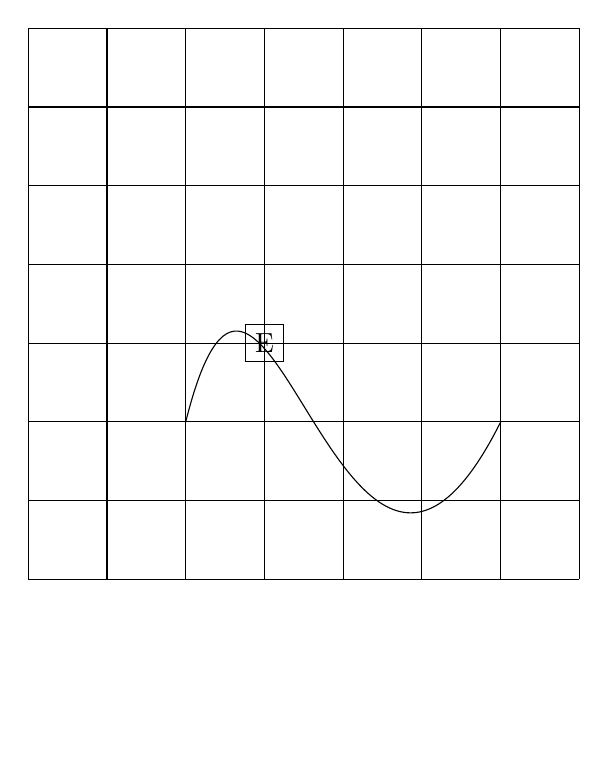
\begin{tikzpicture}
 \node[draw,shape=rectangle] at (1,1) {E};
     \draw (0,0) .. controls (1,4) and (2,-4) .. (4,0);
     \draw (-2,-2) grid (5,5);
\end{tikzpicture}


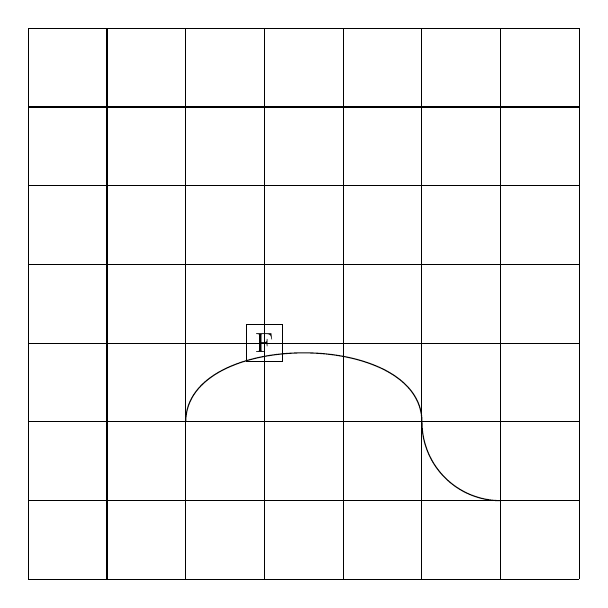
\begin{tikzpicture}
 \node[draw,shape=rectangle] at (1,1) {F};
     \draw (0,0) to [out=90, in=90] (3,0) to [out=-90, in=180] (4,-1);
     \draw (-2,-2) grid (5,5);
\end{tikzpicture}

%y = x^2
\begin{tikzpicture}
 \node[draw,shape=rectangle] at (1,1) {G};
     \draw[->] (0,0) -- (5,0);
     \draw[->] (0,0) -- (0,5);
     \draw[domain=-2:2] plot (\x, {\x*\x});
 \end{tikzpicture}

 \begin{tikzpicture}
  \node[draw,shape=rectangle] at (1,1) {1};
      \draw (0,0) rectangle (4,4);
      \node at (-0.1,-0.1) {O};
      \node at (4.1, -0.1) {A};
      \node at (4.1, 4.1) {B};
      \node at (-.1, 4.1) {C};
 \end{tikzpicture}

\begin{tikzpicture}
 \node[draw,shape=rectangle] at (1,1) {2};
      \draw (0,0) rectangle (4,4);
      \node[below left] at (0,0) {O};
      \node[below right] at (4, 0) {A};
      \node[above right] at (4, 4) {B};
      \node[above left] at (0, 4) {C};
 \end{tikzpicture}

 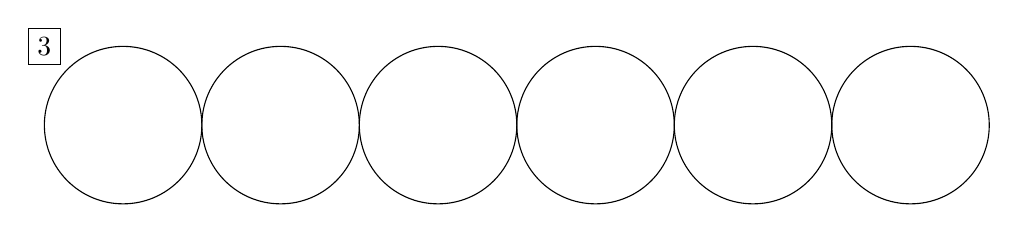
\begin{tikzpicture}
 \node[draw,shape=rectangle] at (1,1) {3};
      \foreach \x in {1,...,6}
      {
         \draw (\x*2,0) circle [radius=1];
      }
 \end{tikzpicture}

 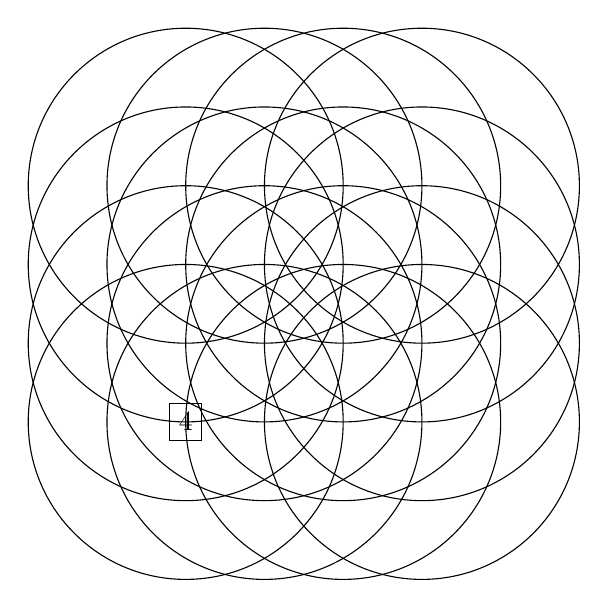
\begin{tikzpicture}
 \node[draw,shape=rectangle] at (1,1) {4};
      \foreach \x in {1,2,3,4}
      {
         \foreach \y in {1,2,3,4}
    	    {
             \draw (\x,\y) circle [radius=2];
         }
      }
 \end{tikzpicture}

 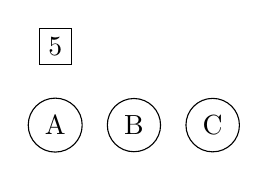
\begin{tikzpicture}
 \node[draw,shape=rectangle] at (1,1) {5};
      \foreach \i\j in {1/A,2/B,3/C}
      {
         \node[draw,shape=circle] at (\i,0) {\j};
      }
 \end{tikzpicture}

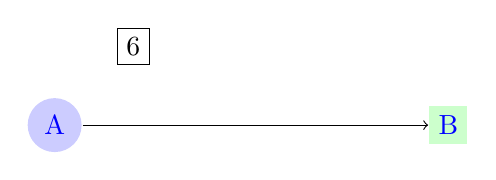
\begin{tikzpicture}
\node[draw,shape=rectangle] at (1,1) {6};
     \node (A) at (0,0) [thick, blue, circle, fill=blue!20]{A};
     \node (B) at (5,0) [thick, blue, rectangle, fill=green!20]{B};
     \draw[->] (A)--(B);
\end{tikzpicture}


\tikzstyle{roundnode}=[circle, draw=green!60, fill=green!5, very thick, minimum size=7mm]
\tikzstyle{squarednode}=[rectangle, draw=red!60, fill=red!5, very thick, minimum size=5mm]
\begin{tikzpicture}
\node[draw,shape=rectangle] at (1,1) {7};
\node[squarednode] (A) {2};
\node[roundnode] (B) [above=of A] {1};
\node[squarednode] (C) [right=of A] {3};
\node[roundnode] (D) [below=of A] {4};

\draw[->] (B.south) -- (A.north);
\draw[->] (A.east) -- (C.west);
\draw[->] (C.south) .. controls +(down:35mm) and +(left:5mm) .. (D.west);
    
\end{tikzpicture}

\lipsum[2]
    
\begin{tikzpicture}
\node[draw,shape=rectangle] at (1,1) {8};
  \draw[->] (-3, 0) -- (4.2, 0) node[right] {$x$};
  \draw[->] (0, -3) -- (0, 4.2) node[above] {$y$};
  \draw[scale=0.5, domain=-3:3, smooth, variable=\x, blue] plot ({\x}, {\x*\x});
  \draw[scale=0.5, domain=-3:3, smooth, variable=\y, red]  plot ({\y*\y}, {\y});
\end{tikzpicture}

\begin{tikzpicture}
\node[draw,shape=rectangle] at (1,1) {9};
\begin{axis}[xmax=20,ymax=20, samples=200]
  \addplot[blue, ultra thick] (x,6*ln(x));
  \addplot[red,  ultra thick] (x*x,x);
\end{axis}
\end{tikzpicture}


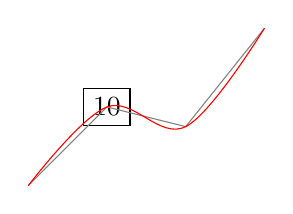
\begin{tikzpicture}
\node[draw,shape=rectangle] at (1,1) {10};
\draw [gray]  (0,0) -- (1,1) -- (2,0.75) -- (3,2);
\draw [red] plot [smooth, tension=0.6] coordinates { (0,0) (1,1) (2,0.75) (3,2)};
\end{tikzpicture}

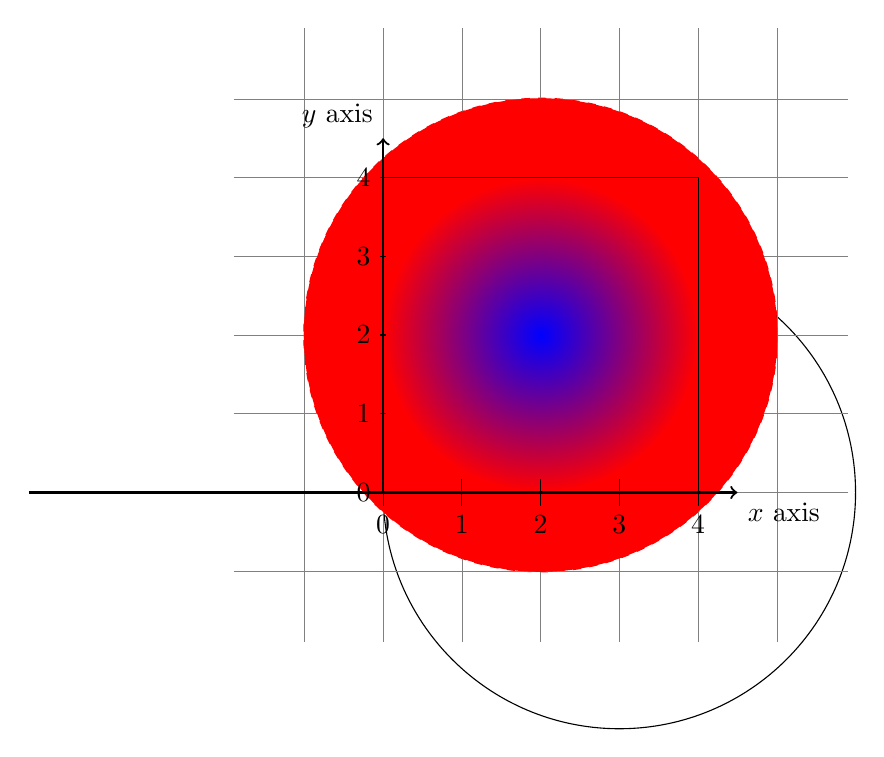
\begin{tikzpicture}

 \draw (0,0) -- (0,4);

 \draw[thick] (0,0) -- (4,4);

 \draw[fill=red] (0,0) rectangle (4,4);

\draw (0,0) parabola (1,4);

 \draw[<->] (0,0) -- (4,4);

 \draw (0,0) .. controls (0,4) and (4,0) .. (4,4);

\draw[red,thick,dashed] (2,2) circle (3cm);

 \draw (2,2) ellipse (3cm and 1cm);

 \draw (3,0) circle (3cm);
 \draw (3,0) arc (0:75:3cm);

 \draw[step=1cm,gray,very thin] (-1.9,-1.9) grid (5.9,5.9);

 \filldraw[red] (2,2) circle (3cm);

 \shadedraw[inner color=blue,outer color=red, draw=black] (0,0) rectangle (4,4);

\draw[thick,->] (-4.5,0) -- (4.5,0) node[anchor=north west] {$x$ axis};
\draw[thick,->] (0,0) -- (0,4.5) node[anchor=south east] {$y$ axis};

 \foreach \x in {0,1,2,3,4}
     \draw (\x cm,5pt) -- (\x cm,-5pt) node[anchor=north] {$\x$};
 \foreach \y in {0,1,2,3,4}
     \draw (1pt,\y cm) -- (-1pt,\y cm) node[anchor=east] {$\y$};

\end{tikzpicture}
\\
\lipsum[2]
\\
\\
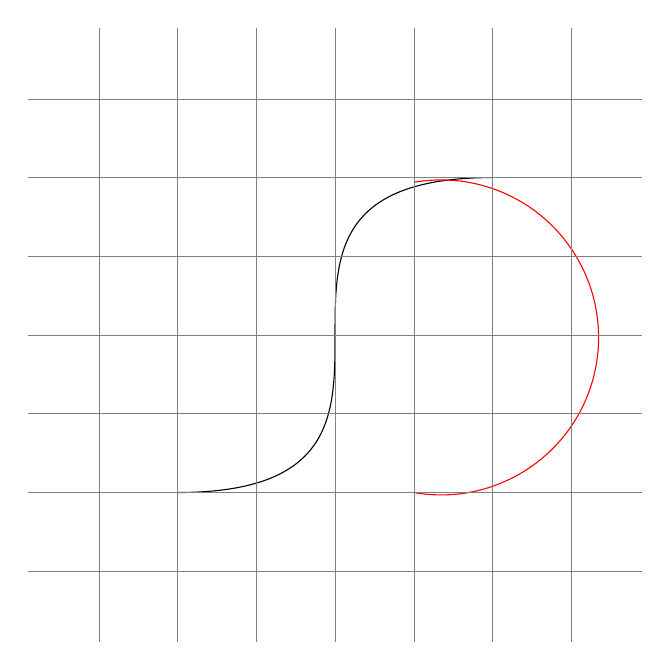
\begin{tikzpicture}
\draw (0,0) .. controls (4,0) and (0,4) .. (4,4);
\draw[red] (3,0) arc (-100:100:2cm);
\draw[step=1cm,gray,very thin] (-1.9,-1.9) grid (5.9,5.9);
\end{tikzpicture}

\tikzstyle{roundnode}=[circle, draw=green!60, fill=green!5, very thick, minimum size=7mm]
\tikzstyle{squarednode}=[rectangle, draw=red!60, fill=red!5, very thick, minimum size=5mm]
\begin{tikzpicture}
\node[squarednode] (A) {2};
\node[roundnode] (B) [above=of A] {1};
\node[squarednode] (C) [right=of A] {3};
\node[roundnode] (D) [below=of A] {4};

\draw[->] (B.south) -- (A.north);
\draw[->] (A.east) -- (C.west);
\draw[->] (C.south) .. controls +(down:35mm) and +(left:5mm) .. (D.west);
    
\end{tikzpicture}

\tikzstyle{startstop} = [rectangle, rounded corners, minimum width=3cm, minimum height=1cm,text centered, draw=black, fill=red!30]
\tikzstyle{io} = [trapezium, trapezium left angle=70, trapezium right angle=110, minimum width=3cm, minimum height=1cm, text centered, draw=black, fill=blue!30]
\tikzstyle{process} = [rectangle, minimum width=3cm, minimum height=1cm, text centered, text width=3cm, draw=black, fill=orange!30]
\tikzstyle{decision} = [diamond, minimum width=3cm, minimum height=1cm, text centered, draw=black, fill=green!30]
\tikzstyle{arrow} = [thick,->,>=stealth]


\begin{tikzpicture}[node distance=2cm]

\node (start) [startstop] {Start};
\node (in1) [io, below of=start] {Input};
\node (pro1) [process, below of=in1] {Process 1};
\node (dec1) [decision, below of=pro1] {Decision 1};
\node (pro2b) [process, right of=dec1, xshift=2cm] {Process 2b};
\node (pro2a) [process, below of=pro2b, yshift=-0.5cm] {Process 2a text text text text text text text text text text};
\node (out1) [io, below of=pro2a] {Output};
\node (stop) [startstop, below of=out1] {Stop};

\draw [arrow] (start) -- (in1);
\draw [arrow] (in1) -- (pro1);
\draw [arrow] (pro1) -- (dec1);
\draw [arrow] (pro2b) -- (pro2a);
\draw [arrow] (dec1) |- node[anchor=east] {yes} (pro2a);
\draw [arrow] (dec1) -- node[anchor=south] {no} (pro2b);
\draw [arrow] (pro2b) |- (pro1);
\draw [arrow] (pro2a) -- (out1);
\draw [arrow] (out1) -- (stop);


\end{tikzpicture}

\tikzstyle{startstop} = [rectangle, rounded corners, minimum width=3cm, minimum height=1cm,text centered, draw=black, fill=red!30]
\tikzstyle{io} = [trapezium, trapezium left angle=70, trapezium right angle=110, minimum width=3cm, minimum height=1cm, text centered, draw=black, fill=blue!30]
\tikzstyle{process} = [rectangle, minimum width=3cm, minimum height=1cm, text centered, text width=5 cm, draw=black, fill=orange!30]
\tikzstyle{decision} = [diamond, minimum width=3cm, minimum height=1cm, text centered, draw=black, fill=green!30]
\tikzstyle{arrow} = [thick,->,>=stealth]
\tikzstyle{roundNode} =[circle, draw=green!60, fill=green!5, very thick, minimum size=7mm]

\begin{tikzpicture}[node distance=2cm]
\node[startstop] (start) {start};
\node[io] (input1) [below of= start] {read income};
\node[io] (input2) [below of= input1] {read cost};
\node[decision] (d1)  [below of= input2,yshift=-30] {income >= cost?};
\node[process] (p1)  [right of= d1,xshift=90] {profit=income-cost};
\node[io] (out1) [below of= p1] {print profit};
\node[process] (p2)  [below of= d1,yshift=-30] {loss=cost-income};
\node[io] (out2) [below of= p2] {print loss};
\node[startstop] (stop) [below of= out2] {end};

\draw[arrow] (start)--(input1);
\draw[->] (input1)--(input2);
\draw[->] (input1)--(input2);
\draw[->] (input2)--(d1);
\draw[->] (d1)--(p1);
\draw[->] (d1)--(p2);
\draw[->] (p1)--(out1);
\draw[->] (p2)--(out2);
\draw[->] (out2)--(stop);
\draw (out1.south)--(5.2,-14);
\draw[->] (5.2,-14)--(stop.east);

\end{tikzpicture}

\begin{tikzpicture}

      \node[roundNode] (n1) {1};
      \node[roundNode] (n2) [below left of=n1,yshift=-5mm] {2};
        \node[roundNode] (n3) [below right of=n1,yshift=-5mm] {3};

        \path
    (n1) edge [loop above] node {0.6} (n1)
        edge [bend right] node {0.4} (n2)
    (n2) edge node [below]{1.0} (n1)
    (n3) edge [loop below] node {0.8} (n3)
        edge node[right] {0.1} (n1)
        edge node[below] {0.1} (n2); 
        
    
\end{tikzpicture}

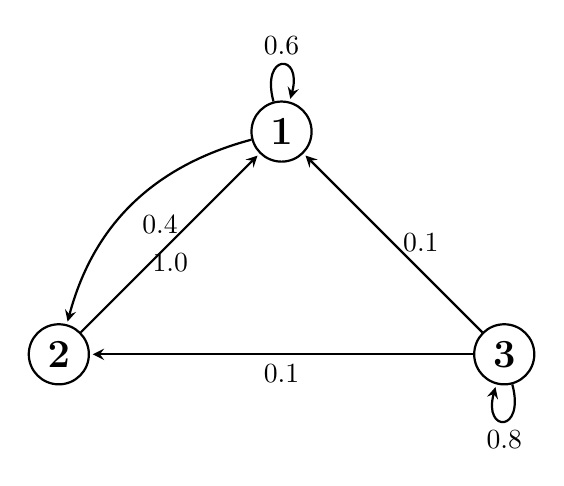
\begin{tikzpicture}[->,>=stealth,shorten >=1pt,auto,node distance=4cm,
                thick,main node/.style={circle,draw,font=\Large\bfseries}]

  \node[main node] (1) {1};
  \node[main node] (2) [below left of=1] {2};
  \node[main node] (3) [below right of=1] {3};

  \path
    (1) edge [loop above] node {0.6} (1)
        edge [bend right] node {0.4} (2)
    (2) edge node [below]{1.0} (1)
    (3) edge [loop below] node {0.8} (3)
        edge node[right] {0.1} (1)
        edge node[below] {0.1} (2);      
\end{tikzpicture}

\newpage
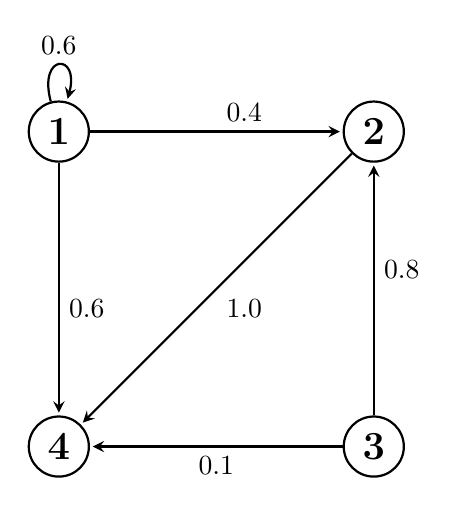
\begin{tikzpicture}[->,>=stealth,shorten >=1pt,auto,node distance=4cm,
                thick,main node/.style={circle,draw,font=\Large\bfseries}]

  \node[main node] (1) {1};
  \node[main node] (2) [right of=1] {2};
  \node[main node] (4) [below  of=1] {4};
  \node[main node] (3) [right of=4] {3};

  \path
    (1) edge [loop above] node {0.6} (1)
        edge [below right] node {0.6} (4)
        edge [ above right ] node {0.4} (2)
    (2) edge node [bend left]{1.0} (4)
    (3) edge [above right] node {0.8} (2)
        edge node[below] {0.1} (4)
    (4)  ;      
\end{tikzpicture}
\newpage
\begin{figure}
    \centering
    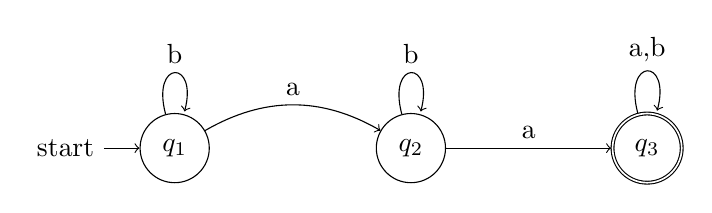
\begin{tikzpicture}[->, node distance = 3cm]
    \node[initial, state] (A) {$q_1$};
    \node[state](B) [right of = A] {$q_2$};
    \node[state, accepting] (C) [right of = B] {$q_3$};
    \path (A) edge [loop above] node{b} (A);
    \path (A) edge [bend left][above] node {a} (B);
    \path (B) edge [above] node {a} (C);
    \path (B) edge [loop above] node {b} (B);
    \path (C) edge [loop above] node {a,b} (C);
    \end{tikzpicture}
    \caption{Automaton}
    \end{figure}

    \begin{figure}
        \centering
        
 
    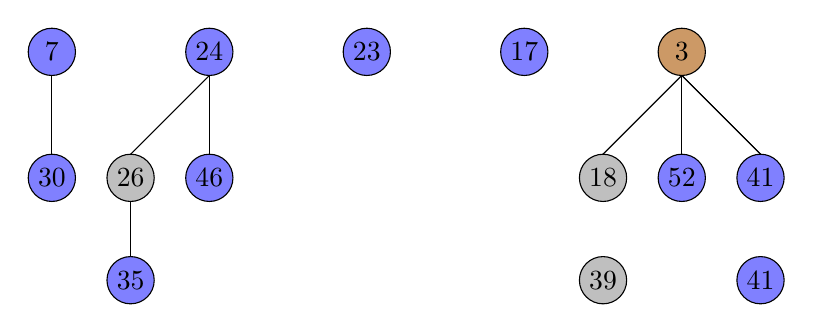
\begin{tikzpicture}
        \draw [fill=blue!50] (0, -7.7) circle (0.3cm) node {7};
        
        \draw [fill=blue!50] (0, -9.3) circle (0.3cm) node {30};
        \draw [fill=blue!50] (2, -9.3) circle (0.3cm) node {46};
        \draw [fill=gray!50] (1, -9.3) circle (0.3cm) node {26}; 
        \draw [fill=blue!50] (1, -10.6) circle (0.3cm) node {35};
        \draw [fill=blue!50] (4, -7.7) circle (0.3cm) node {23};
        \draw [fill=blue!50] (6, -7.7) circle (0.3cm) node {17};
        \draw [fill=blue!50] (2, -7.7) circle (0.3cm) node {24};
        \draw [fill=brown!80] (8, -7.7) circle (0.3cm) node {3};
        \draw [fill=blue!50] (8, -9.3) circle (0.3cm) node {52};
        
        \draw [fill=gray!50] (7, -9.3) circle (0.3cm) node {18};

        \draw [fill=gray!50] (7, -10.6) circle (0.3cm) node {39};
        
        \draw [fill=blue!50] (9, -9.3) circle (0.3cm) node {41};
        \draw [fill=blue!50] (9, -10.6) circle (0.3cm) node {41};
        
        
        \draw (2, -8) -- (2, -9);
        \draw (0, -8) -- (0, -9);
        \draw (2, -8) -- (1, -9);
        \draw (1, -9.6) -- (1, -10.3);
        
        
        
        
        \draw (8, -8) -- (8, -9);
        
        \draw (7, -9) -- (8, -8);
        \draw (9, -9) -- (8, -8);
        \draw (9, -9) -- (8, -8);
        
        
        
    \end{tikzpicture}
\caption{Caption}
        \label{fig:my_label}
           \end{figure}

\end{document}